\chapter{Proses Bisnis dan Pengumpulan Data Fisik}

\section{Proses Bisnis}
Sebelum menganalisa untuk perancangan sistem database maka kita membutuhkan beberapa berkas untuk kita analisis dan berkas-berkas tersebut ada dalam proses bisnis pembuatan SIM sebagai berikut :
\begin{enumerate}
	\item Yang pertama adalah fotokopi KTP dengan menyiapkan beberapa lembar fotokopi. Anda perlu mencari tempat fotokopi KTP terdekat dengan lokasi Anda saat ini;

	\item Surat Keterangan Sehat Jasmani dan Rohani,
    Surat ini biasanya dapat dibuat di klinik kepolisian atau di pusat pelayanan kesehatan yang merupakan keterangan dari dokter;

	\item •	Registrasi dan Isi Formulir Pendaftaran
	Beli formulir permohonan pembuatan SIM sesuai dengan tarif yang telah ditentukan. Anda juga dapat membayar premi asuransi sebesar Rp 30.000. Kemudian isi formulir pendaftaran tersebut sesuai data pribadi Anda yang benar. Kemudian serahkan fomulir tersebut ke petugas loket yang telah disediakan. Tunggu nama Anda dipanggil oleh petugas loket tersebut;

	\item Mengikuti Ujian
	Terdapat dua tahap ujian yang harus Anda lakukan dalam permohonan pembuatan SIM, antara lain:
	Ujian Teori: Jika Anda lulus, Anda akan menjalani ujian selanjutnya yaitu ujian praktik.
	Ujian Praktik: Jika lulus, SIM Anda akan diproduksi atau dicetak.
	Namun jika tidak lulus pada salah satu dari kedua tes tersebut, Anda diperbolehkan mengulang setelah tenggang 7 hari, 14 hari, dan 30 hari. Sama seperti untuk ujian teori, jika Anda mengulang ujian praktik lalu tidak lulus, tidak mengulang, tidak datang kembali, atau tidak ada keterangan, uang yang telah dibayarkan akan dikembalikan;

    \item Melakukan Proses Identifikasi
    Dalam proses ini, Anda akan diminta untuk melakukan pemotretan foto SIM, membubuhkan tanda tangan serta sidik jari pada sistem komputer dimana akan secara otomatis menjadi bagian dari identitas pribadi Anda;

    \item Ambil SIM
    Anda hanya perlu menunggu hingga nama Anda dipanggil untuk mengambil SIM yang sudah jadi di loket pengambilan SIM;
    
   
	
	\begin{figure}[H]
		\centering
		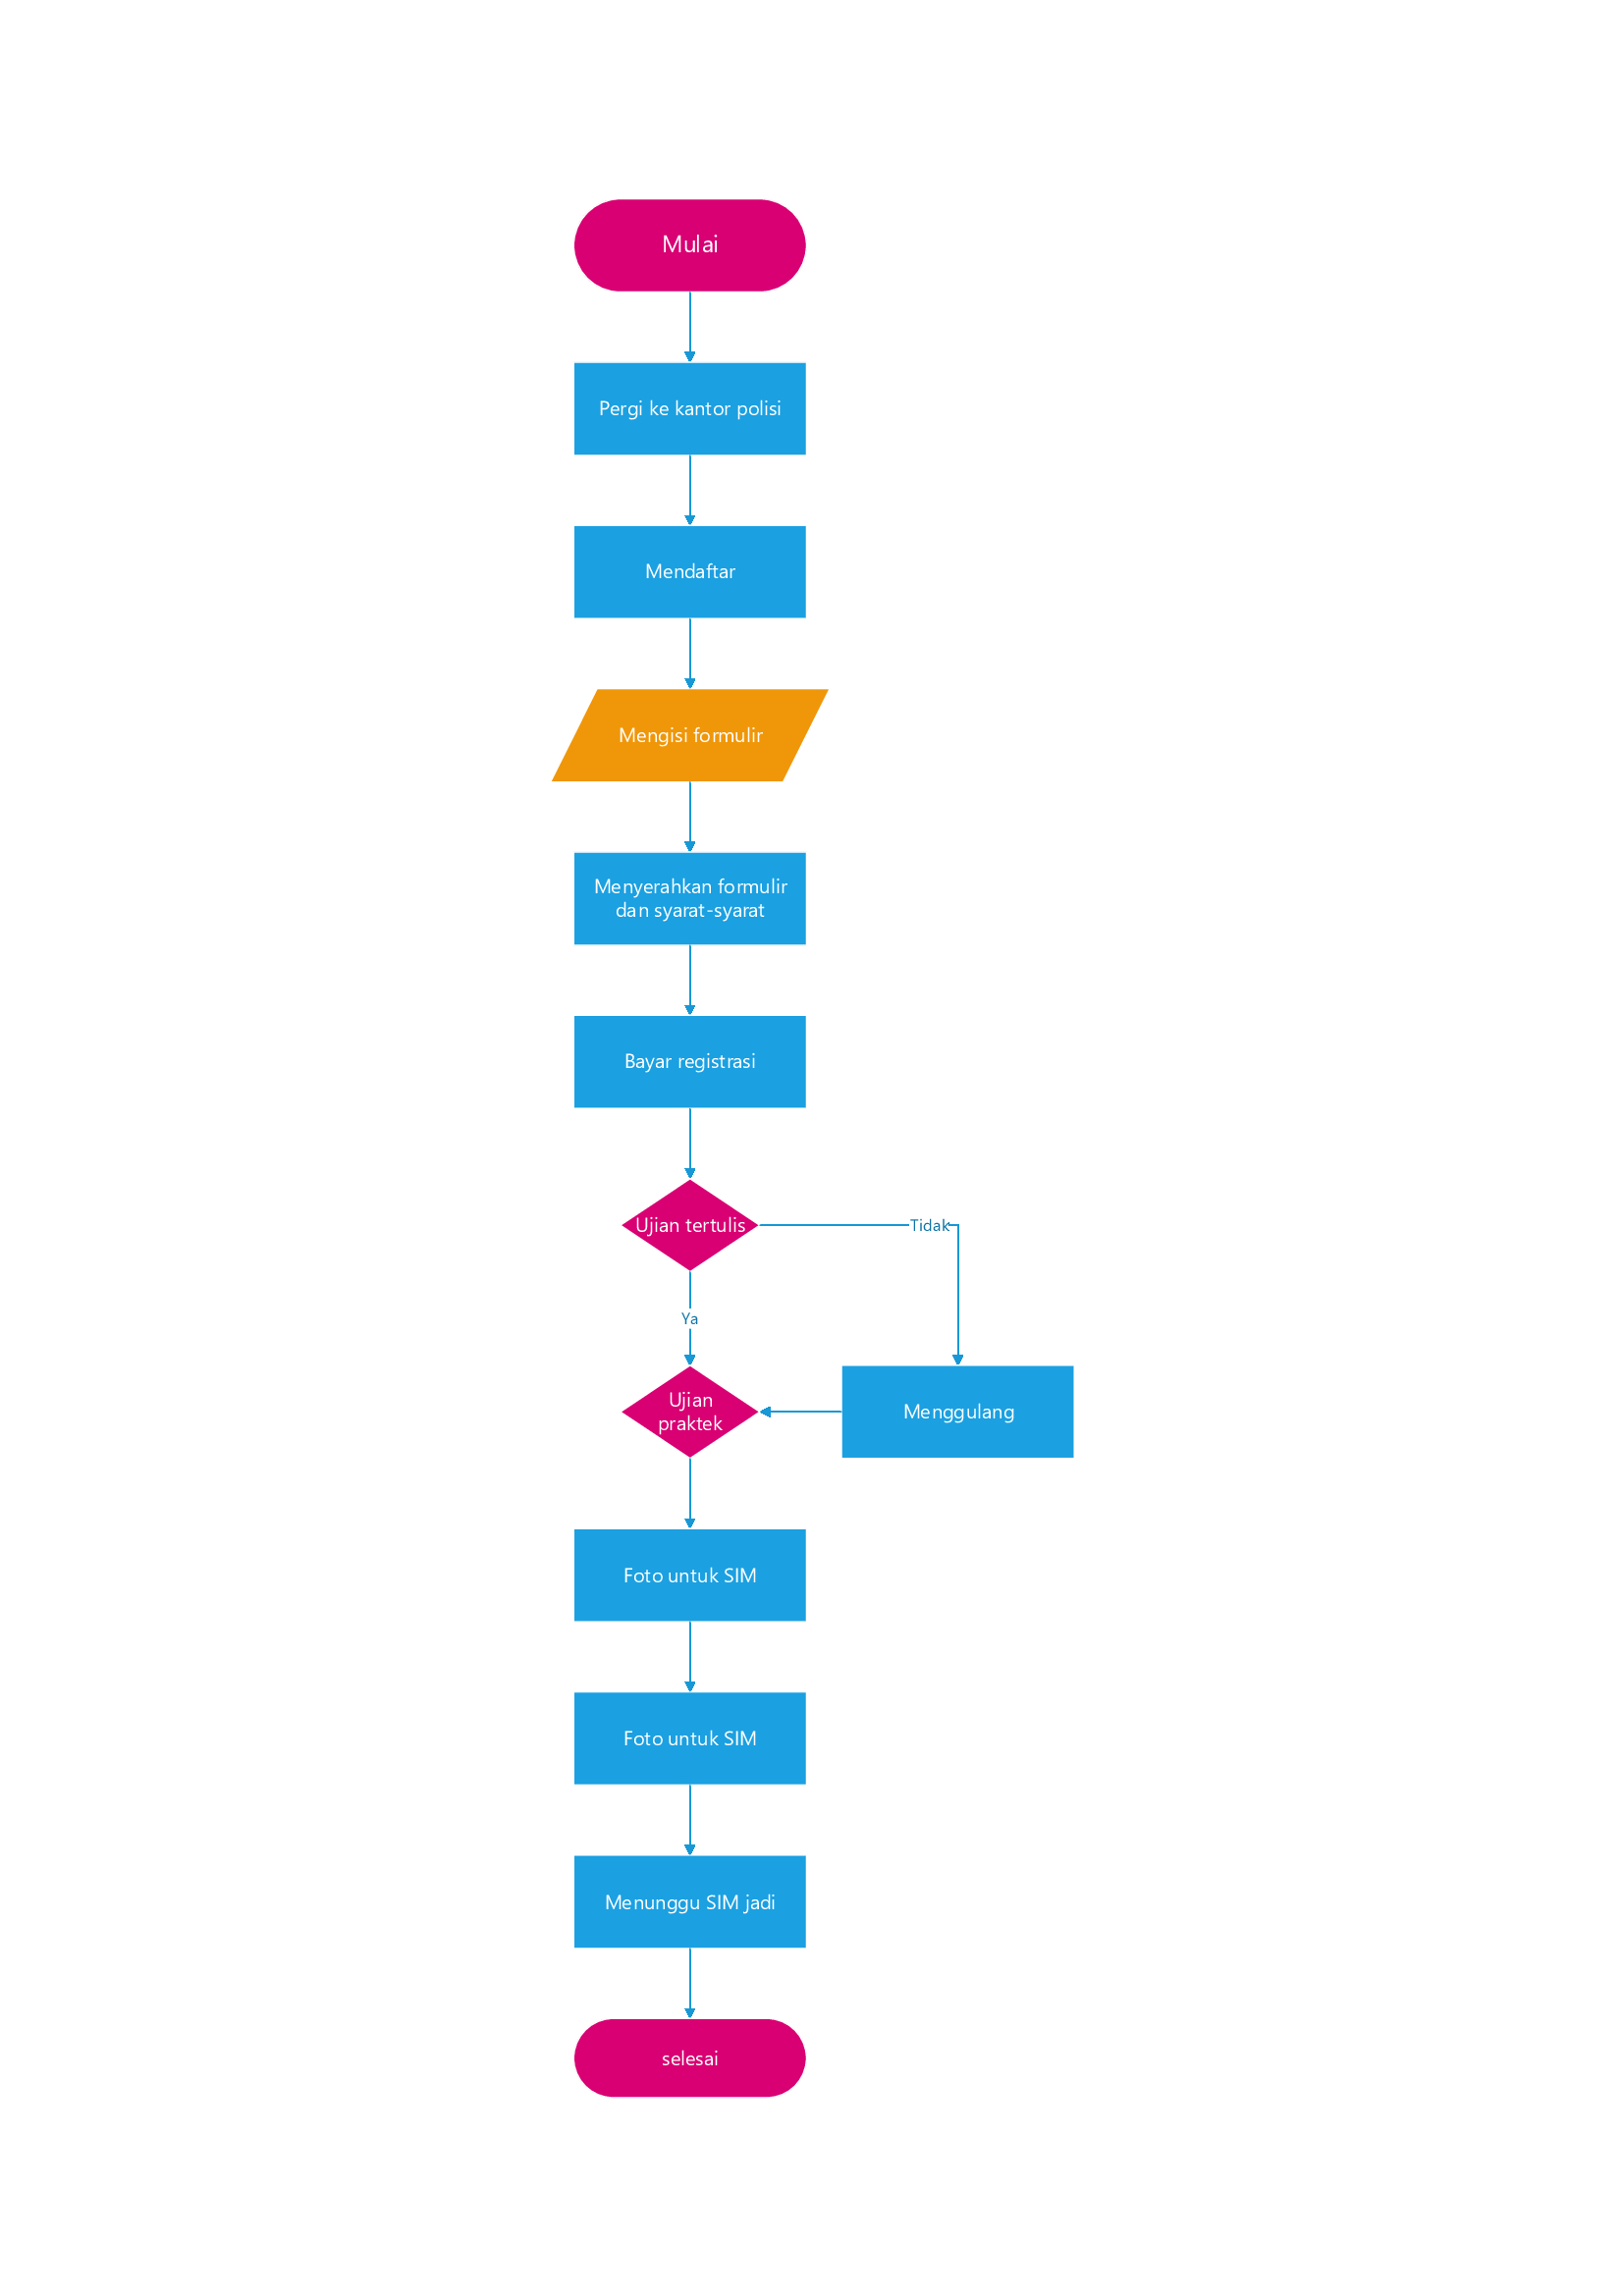
\includegraphics[width=16cm]{figures/simflow2.jpg}
		\caption{Flowmap Prosedur Pembuatan SIM}	
	\end{figure}
\end{enumerate}
\subsection{Syarat-Syarat membuat SIM}
\begin{enumerate}
\item Surat permohonan pembuatan SIM;
a. identitas diri berupa Kartu Tanda Penduduk;
b. pengisian formulir permohonan;
c. rumusan sidik jari;
\item Surat Kesehatan untuk memperoleh Surat Izin Mengemudi (SIM);
a. sehat jasmani dengan surat keterangan dari dokter;
b. sehat rohani dengan surat lulus tes psikologis;
\item Surat lulus ujian untuk memperoleh Surat Izin Mengemudi (SIM) perorangan ;
a. ujian teori;
b. ujian praktik; dan/atau;
c. ujian keterampilan melalui simulator;
\section{Surat Izin Mengemudi (SIM) golongan B I dan B II perorangan juga harus mememenuhi persyaratan sebagai berikut}
a. Untuk memperoleh SIM B I harus memiliki SIM A sekurang-kurangnya 12 bulan;
b. Untuk memperoleh SIM B II harus memiliki SIM B I sekurang-kurangnya 12 bulan;
\section{Tarif Pembuatan SIM baru dan perpanjangan}
a.Biaya pembuatan SIM A baru adalah RP. 120.000,- dan perpanjangan adalah Rp. 80.000,-;
b.Biaya pembuatan SIM BI baru adalah RP. 120.000,- dan perpanjangan adalah Rp. 80.000,-;
c.Biaya pembuatan SIM B II baru adalah RP. 120.000,- dan perpanjangan adalah Rp. 80.000,-;
d.Biaya pembuatan SIM C baru adalah RP. 100.000,- dan perpanjangan adalah Rp. 75.000,-;
e.Biaya pembuatan SIM D baru adalah RP. 50.000,- dan perpanjangan adalah Rp. 30.000,-;


Data fisik sangat dibutuhkan untuk membuat SIM(
Surat Izin Mengemudi), adapun Bukti fisiknya sebagai berikut :  
\end{enumerate}
\begin{enumerate}

	\item Kartu Tanda Penduduk(KTP)
	\begin{figure}[H]
		\centering
		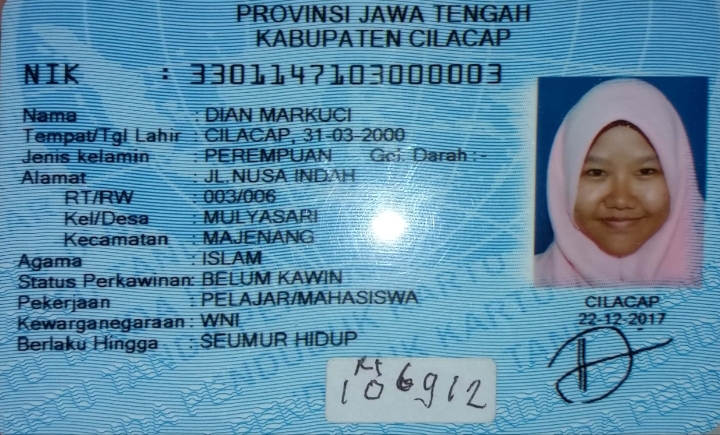
\includegraphics[width=12cm]{figures/KTP.jpeg}
		\caption{Kartu Tanda Penduduk.}	
	\end{figure}

\end{enumerate}